\documentclass[Preamble]{subfiles}
\begin{document}

\chapter{Domain Name System}


Domain Name System, DNS, is used to find IP-addresses from a logical name using the concept of the Host Lookup Table.
The Host Lookup Table, HLT, was a file placed on every computer connected to the network which contained the IP-address and the logical name for each computer connected.

When the HLT was updated, all computers needed to add the address which, due to the expansion of the university's increasingly connecting computers to the network, became an obstacle and hindrance for the flow.
To solve this, the DNS system was founded in 1985.

DNS is like a big telephone book which everyone uses to lookup IP-addresses by logical name, through an A-record, rather than everyone keeping track of all connected addresses.



\section{DNS fundamentals}
To find the computer's host name the command \code{hostname} will show the human logic readable name for the computer.
This is what will be shown on a search on the network where the computer is connected.
\\
\\
In Linux one can run the \code{nm-tool} will access the NetworkManager Tool and show the IP-address, MAC-address, connection state and DNS-server for the computer.
This is shown on figure \ref{fig:nm-tool}\footnote{Note that this is on a virtual machine which do not show as much as a native Linux machine will}.
\\
You can run a similar command in Windows run \code{ipconfig /all} to access IP-address, DNS-server, MAC-Address\dots -- shown on figure \ref{fig:ipconfig}.


\begin{figure}[hbtp]
\centering
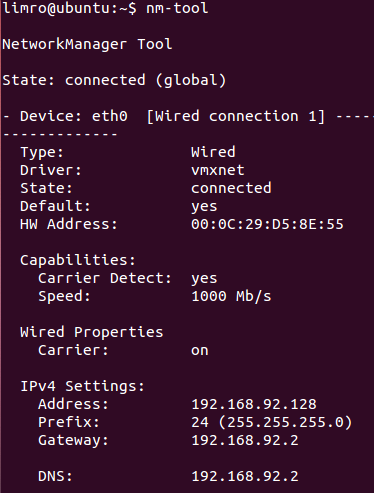
\includegraphics[scale=0.7]{nm-tool.png}
\caption{Use of the command \code{nm-tool}}
\label{fig:nm-tool}
\end{figure}



\begin{figure}[hbtp]
\centering
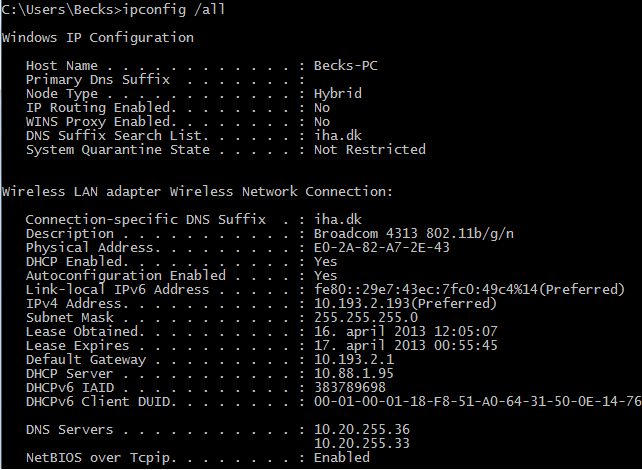
\includegraphics[scale=0.7]{ipconfig.png}
\caption{Use of the command \code{ipconfig /all}}
\label{fig:ipconfig}
\end{figure}

To locate an IP-address and the latency use the \code{ping} command.
\code{ping} will target either a webserver name to get the IP-address or target the IP-address directly without asking the DNS-server.
This is shown on figure \ref{fig:ping}


\begin{figure}[hbtp]
\centering
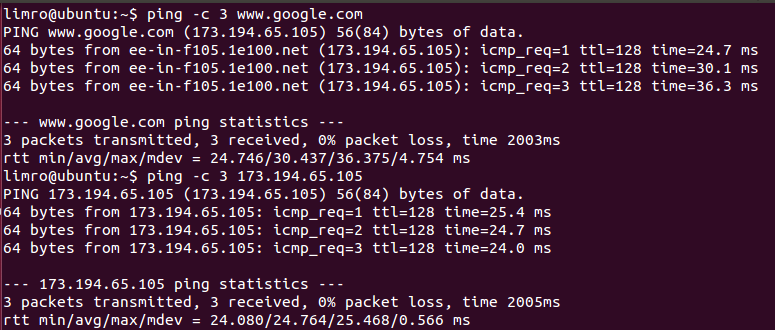
\includegraphics[scale=0.7]{ping}
\caption{Use of the command \code{ping -c 3 www.google.com}}
\label{fig:ping}
\end{figure}


To make a redirection or a shortcut the address in the file \textit{/etc/hosts} can be changed so it will take a alias in a browser and redirect this to an IP-address. Other records can also be added to li


When requesting a webserver through a DNS, the root servers first redirect to the Top-Level Domain server, TLD, which contains the '.com', '.net', '.dk' etc.
From here the domain server can return IP for name server, to which the client can call. 
This will then (most likely) recursively or (less likely)iterative return the specified IP-address to the client.


If requesting a company's domain the client will be directed to a DNS zone which, in this case, will be for the English version of the website and ftp-server or the Danish version of the website and ftp-server.
Each one is a zone, placed different places and with its own administration and a server can contain multiple zones.







\end{document} 